% Ten-minute presentation; nine main slides and three optional backup slides.
% Source: current configs/dns384.json, architecture-primer.md, and verified GPU test.
% Editable metadata below. The scientific content is filled in, not a blank template.
% Compile twice: pdflatex -halt-on-error lapflow-10-minute-presentation.tex
% Speaker notes are embedded but hidden in the audience PDF.
% See lapflow-10-minute-speaker-notes.md for the timing and spoken explanation.
\documentclass[aspectratio=169,11pt]{beamer}
\usepackage{amsmath,amssymb,booktabs,tabularx,tikz}
\usetikzlibrary{arrows.meta,positioning}
\usetheme{default}
\definecolor{navy}{RGB}{25,49,76}
\definecolor{teal}{RGB}{0,117,124}
\definecolor{amber}{RGB}{165,94,20}
\definecolor{muted}{RGB}{90,101,112}
\setbeamercolor{structure}{fg=navy}
\setbeamercolor{frametitle}{fg=navy}
\setbeamercolor{block title}{fg=white,bg=navy}
\setbeamercolor{block body}{bg=navy!5}
\setbeamercolor{alerted text}{fg=amber}
\setbeamertemplate{navigation symbols}{}
\setbeamertemplate{itemize items}[circle]
\setbeamertemplate{footline}{\hfill\color{muted}\scriptsize\insertframenumber/9\hspace{0.45cm}\vspace{0.2cm}}
\setbeameroption{hide notes}
\pdfstringdefDisableCommands{\def\translate#1{#1}}
\newcolumntype{Y}{>{\raggedright\arraybackslash}X}
\setlength{\tabcolsep}{5pt}
\tikzset{
  box/.style={draw=navy!55,rounded corners=2pt,fill=navy!4,align=center,
              minimum height=1cm,text width=2.3cm,font=\small},
  band/.style={box,draw=teal!70,fill=teal!7},
  arr/.style={-{Latex[length=2mm]},thick,draw=navy!70}}
\newcommand{\keypoint}[1]{\begin{block}{}#1\end{block}}
\newcommand{\smallsource}[1]{\vfill{\tiny\color{muted}#1}}
\title{Generating 3D turbulent velocity fields}
\subtitle{The encoder bottleneck and a LapFlow baseline}
\author{\textit{Your name}} % Replace with your name.
\institute{\textit{Your laboratory}} % Replace or remove.
\date{\textit{Presentation date}} % Replace before presenting.

\begin{document}

% 1. 0:00--0:20
\begin{frame}
  \titlepage
  \note{This is a method-development update about unconditional generation of
  three-dimensional turbulent velocity snapshots. I will focus on why the
  representation is difficult and what multiscale flow matching actually learns.}
\end{frame}

% 2. 0:20--1:00
\begin{frame}{The question: can we generate realistic spatial statistics?}
  \begin{itemize}
    \item Data: one joint $(u,v,w)$ velocity field on a $384^3$ DNS grid.
    \item Output: a new snapshot drawn from a learned distribution.
    \item Evaluate energy, spectra, velocity PDFs, and divergence.
  \end{itemize}
  \medskip
  \begin{center}
    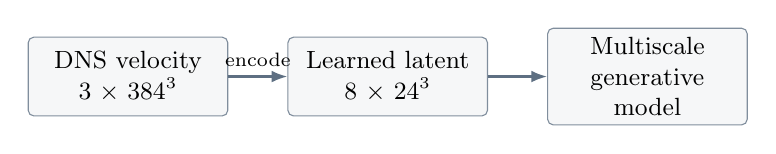
\begin{tikzpicture}[node distance=0.75cm]
      \node[box] (u) {DNS velocity\\$3\times384^3$};
      \node[box,right=of u] (z) {Learned latent\\$8\times24^3$};
      \node[box,right=of z] (g) {Multiscale\\generative model};
      \draw[arr] (u)--node[above,font=\scriptsize]{encode} (z);
      \draw[arr] (z)--(g);
    \end{tikzpicture}
  \end{center}
  \keypoint{First learn a representation; then learn to generate it.}
  {\small\color{muted}Current scope: unconditional snapshots; no physical-time forecast.}
  \note{The data are velocity volumes, not RGB images or independent 2D slices.
  There is no input history, pressure channel, or physical-time condition in this
  baseline. The challenge has two parts: compress a field without discarding its
  important structure, then learn the distribution of the compressed fields.
  Matching these spatial diagnostics would not establish temporal dynamics.}
\end{frame}

% 3. 1:00--2:20
\begin{frame}{Why we chose a small 3D encoder}
  \begin{columns}[T]
    \begin{column}{0.53\textwidth}
      \textbf{The memory problem}
      \begin{itemize}
        \item One FP32 velocity volume: $648$ MiB.
        \item Illustrative full-grid feature tensor:\\
              $128\times384^3$ FP32 values $=27$ GiB.
        \item Training also needs activations, gradients, and optimizer state.
      \end{itemize}
    \end{column}
    \begin{column}{0.43\textwidth}
      \textbf{Our initial choices}
      \begin{itemize}
        \item Downsample in the first convolution.
        \item Small feature widths; train local crops.
        \item Deterministic autoencoder trained on DNS.
      \end{itemize}
    \end{column}
  \end{columns}
  \medskip
  \keypoint{A deliberate low-memory starting point, with a substantial fidelity risk.}
  {\small A 3D VAE is possible. Variational training alone would not remove the compression bottleneck.}
  \note{A raw field is manageable, but a hidden feature volume can be much larger.
  The 27 GiB example is illustrative, not an allocation made by our current model.
  Previous memory problems motivated prioritizing a working low-memory baseline.
  We immediately stride the encoder, use small channel counts, and tile the
  computation. We did not reuse an image VAE unchanged: our representation is a
  separately trained deterministic 3D autoencoder. A 3D VAE remains possible; it
  would add posterior sampling and KL regularization. We have not demonstrated
  that the present representation is scientifically adequate or optimal.}
\end{frame}

% 4. 2:20--3:35
\begin{frame}{What the encoder and decoder actually learn}
  \small
  \begin{tabularx}{\linewidth}{lYY}
    \toprule
    Component & Transformation & Purpose \\
    \midrule
    Encoder & Four $3^3$ convolutions, stride 2; then $1^3$ projection &
    Combine local velocity patterns into compact learned features \\
    Channels / grids & $3\to8\to16\to24\to32\to8$; $384\to192\to96\to48\to24\to24$ &
    Reduce spatial cost while building features \\
    Decoder & $8\to32$ projection; four transposed convolutions back to $3\times384^3$ &
    Learn how to reconstruct velocity from those features \\
    \bottomrule
  \end{tabularx}
  \medskip
  \[
    L_{\mathrm{AE}}=\operatorname{mean}_{\mathrm{core}}
      \bigl[D_{\phi}(E_{\psi}(\widetilde U))-\widetilde U\bigr]^2
  \]
  Encoder and decoder train together; both are frozen before flow training.
  \keypoint{Latent channels are learned features. The decoder is a learned reconstruction, not an exact inverse.}
  \smallsource{Encoder: 35,552 parameters. Encoder + decoder: 119,347 parameters.}
  \note{A convolution takes weighted combinations of neighboring velocities and
  applies a nonlinearity. It may learn averages, differences, or more complex
  patterns, but we do not prescribe a physical meaning to a channel. Every
  stride-two layer halves each spatial dimension. The final one-by-one projection
  mixes 32 features into eight at each latent location. The decoder learns
  overlapping contributions to a finer grid using transposed convolutions.
  Reconstruction error teaches both halves which information is useful.
  Velocity is normalized per component using training statistics. We train on
  128-cubed inputs and score 64-cubed cores.}
\end{frame}

% 5. 3:35--4:50
\begin{frame}{The struggle: output resolution is not retained information}
  \[
    \frac{3\,384^3}{8\,24^3}=\boxed{1536\times\text{ fewer scalar values}}
  \]
  \begin{itemize}
    \item Fine velocity differences must survive this bottleneck to be reconstructed.
    \item Squared reconstruction loss can favor smoothing ambiguous detail.
    \item No spectral, gradient, or incompressibility constraint is imposed.
    \item The frozen decoder limits which fields the generator can express.
  \end{itemize}
  \keypoint{Check DNS $\rightarrow$ encoder $\rightarrow$ decoder before judging the generator.}
  \begin{center}
    \small Compare reconstruction spectra and energy, alongside pointwise error.
  \end{center}
  \note{The output again has 384-cubed points, but that is an array size, not a
  guarantee of DNS fidelity. In a severe bottleneck, distinct fine structures
  may receive similar descriptions. A deterministic decoder optimized with
  squared error tends toward their conditional average, which can suppress
  fluctuations. This is a risk to test, not an observed conclusion about the
  fully trained model. The flow model cannot update the frozen representation.
  Tiling uses periodic halos and a single joint latent volume, avoiding independent
  patch generation. Memory efficiency is helpful, but it does not establish
  physical accuracy. A VAE would not automatically recover discarded detail.}
\end{frame}

% 6. 4:50--6:10
\begin{frame}{LapFlow separates the latent into approximation and detail}
  \begin{columns}[T]
    \begin{column}{0.55\textwidth}
      \[
      \begin{aligned}
        M &= P(Z)                 &&(12^3)\\
        C &= P(M)                 &&(6^3)\\
        R &= M-A(C)               &&(12^3)\\
        F &= Z-A(M)               &&(24^3)
      \end{aligned}
      \]
      \small $P$: $2^3$ average pooling.\\
      $A$: nearest-neighbor upsampling.
    \end{column}
    \begin{column}{0.41\textwidth}
      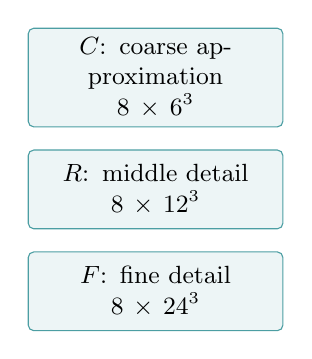
\begin{tikzpicture}[node distance=0.28cm]
        \node[band,text width=3cm] (c) {$C$: coarse approximation\\$8\times6^3$};
        \node[band,text width=3cm,below=of c] (r) {$R$: middle detail\\$8\times12^3$};
        \node[band,text width=3cm,below=of r] (f) {$F$: fine detail\\$8\times24^3$};
      \end{tikzpicture}
    \end{column}
  \end{columns}
  \[
    Z=A\bigl(A(C)+R\bigr)+F
  \]
  \keypoint{Exact recombination of the latent; no additional loss when all bands are retained.}
  {\small\color{muted}These are latent bands, not literal physical Fourier shells or a PDE Laplacian.}
  \note{The encoder learns a lossy representation; this next operation is fixed
  and exactly reversible. Average to make a coarser approximation, expand it,
  and subtract to retain what it missed. Repeat once more. For intuition,
  [2,4,8,10] averages to [3,9], expands to [3,3,9,9], and leaves residual
  [-1,1,-1,1]. Adding them recovers the original. Our decomposition operates on
  learned latent channels, not directly on physical velocity Fourier modes.
  Fine here means detail within the 24-cubed latent, not all DNS-scale detail.
  Use P for pooling to avoid confusing it with the learned decoder.}
\end{frame}

% 7. 6:10--7:30
\begin{frame}{One coupled model predicts transport velocities for the bands}
  \[
    \begin{aligned}
      \dot x_C &= v_C(x_C,\tau),\\
      \dot x_R &= v_R(x_C,x_R,\tau),\\
      \dot x_F &= v_F(x_C,x_R,x_F,\tau).
    \end{aligned}
  \]
  \begin{itemize}
    \item Fine queries inspect all scales; coarse queries inspect only coarse tokens.
    \item Separate scale-specific weights; attention couples their representations.
    \item Sum active velocity losses; one backward pass and optimizer update.
  \end{itemize}
  \keypoint{Fine-scale errors can train coarse features that supply attention keys and values.}
  {\small\color{muted}Here velocity means movement in latent space with generation time $\tau$.}
  \smallsource{Six blocks; width 192; three heads. $2^3$ patches give 27 / 216 / 1,728 tokens.}
  \note{The dots are derivatives with respect to generation time, not DNS time.
  These are noisy evolving band states. A fine token compares its query to coarse,
  middle, and fine keys, then aggregates their values to predict its update.
  Coarse cannot inspect finer states. The information direction is coarse to fine,
  while gradients flow backward: a fine loss can improve coarse internal features.
  It does not directly train the final coarse velocity-output head.
  The sum of scale losses trains a connected model, not three independently trained
  generators. The causal pattern is across scales, not physical time, and does
  not enforce an energy cascade. Each active band stays on its own grid.}
\end{frame}

% 8. 7:30--8:30
\begin{frame}{Generate coarse structure and introduce detail progressively}
  \small
  \begin{tabularx}{\linewidth}{lYY}
    \toprule
    Generation interval & Active ODE states & New state at interval start \\
    \midrule
    $0\to1/3$ & Coarse & $x_C(0)=\epsilon_C$ \\
    $1/3\to2/3$ & Coarse + middle & $x_R(1/3)=\tfrac23\epsilon_R$ \\
    $2/3\to1$ & All three & $x_F(2/3)=\tfrac13\epsilon_F$ \\
    \bottomrule
  \end{tabularx}
  \medskip
  \begin{itemize}
    \item Training learns transport from sampled noisy examples with known derivatives.
    \item Sampling integrates the learned ODE; active coarse bands keep evolving.
    \item Recombine bands, undo latent normalization, then decode one joint field.
  \end{itemize}
  \keypoint{Noise seeds provide diversity; generation steps are not physical timesteps.}
  \smallsource{Current sampler: 48 Heun steps / 96 network evaluations. Independent noise per band.}
  \note{There are three distinct phases, but no coarse representation is discarded
  or replaced by an upsampled noisy state. New residual coordinates activate while
  existing coordinates continue evolving. This differs from Pyramid Flow's
  changing-resolution state and corrective renoising transitions. Our noises are
  sampled once, not injected at every solver step. Heun evaluates a slope,
  predicts an endpoint, and corrects using a second slope. Finally add the bands,
  undo latent normalization, decode, and restore physical units. Training samples
  path points; it does not differentiate through these 48 sampling steps.}
\end{frame}

% 9. 8:30--10:00
\begin{frame}{What is verified, and what would count as a useful result?}
  \small
  \begin{columns}[T]
    \begin{column}{0.48\textwidth}
      \textbf{Execution evidence}
      \begin{itemize}
        \item Actual Perlmutter GPU test at full $384^3$ geometry.
        \item Training, checkpoints, reconstruction, generation, and report completed.
        \item Restart and real-data reader checks passed.
      \end{itemize}
      {\footnotesize Three updates/model; one snapshot/split. Execution test only.}
    \end{column}
    \begin{column}{0.48\textwidth}
      \textbf{Scientific questions}
      \begin{itemize}
        \item Does reconstruction retain energy across scales?
        \item Do generated spectra, energy, and PDFs match held-out DNS?
        \item Are divergence and diversity acceptable?
      \end{itemize}
    \end{column}
  \end{columns}
  \medskip
  \keypoint{First establish what the representation retains; then evaluate generation.}
  {\small\color{muted}This is a 3D adaptation; physical fidelity remains an open question.}
  \note{The original nine-hour job failed because wrapped NetCDF index arrays caused
  millions of library-level reads. The repair uses contiguous blocks and early
  recovery checkpoints. An actual GPU acceptance job completed the entire pipeline
  and a second invocation verified restart behavior. That does not certify model
  quality or long-run completion. Scientific evaluation should first compare DNS
  and its own autoencoder reconstruction, then compare generated and held-out
  ensembles. Energy spectra and divergence are diagnostics, not enforced losses.
  If compression is poor, changing the generative model alone may not help. The
  next architecture choice should follow that evidence; no stronger physical or
  temporal claim is justified yet.}
\end{frame}

% Optional questions only; outside the ten-minute route.
\appendix
\setbeamertemplate{footline}{\hfill\color{muted}\scriptsize Technical backup\hspace{0.45cm}\vspace{0.2cm}}

\begin{frame}{Backup: the exact flow-matching target}
  \small
  For clean band $z_i\in\{C,R,F\}$, noise $\epsilon_i$, and start $a_i$:
  \[
    x_i(\tau)=\frac{\tau-a_i}{1-a_i}z_i+(1-\tau)\epsilon_i,
    \qquad
    b_i=\frac{d x_i}{d\tau}=\frac{z_i}{1-a_i}-\epsilon_i.
  \]
  \[
    L_{\mathrm{flow}}=\sum_{i\ \mathrm{active}}
       \operatorname{mean}\bigl[v_{\theta,i}(x_{\mathrm{active}},\tau)-b_i\bigr]^2.
  \]
  \begin{itemize}
    \item Active count $m$ sampled uniformly from $\{1,2,3\}$;
          $\tau\sim\mathcal U(a_{m-1},1)$ with zero-based $a$.
    \item Coarse appears every update; middle $2/3$; fine $1/3$.
    \item Equal loss coefficients do not imply equal scale influence.
    \item No physical-velocity, spectrum, or PDE loss in flow training.
  \end{itemize}
\end{frame}

\begin{frame}{Backup: a VAE and tiling address different issues}
  \small
  \begin{tabularx}{\linewidth}{lYY}
    \toprule
    Choice & What it changes & What it does not establish \\
    \midrule
    Deterministic AE & One encoded latent; reconstruction loss & Adequate compression fidelity \\
    3D VAE alternative & Posterior mean/variance, sampling, KL penalty & Recovery of discarded detail or incompressibility \\
    Periodic halo tiling & Local computation with context; one joint latent & Physical quality of reconstruction \\
    \bottomrule
  \end{tabularx}
  \medskip
  Current training: $128^3$ input, $64^3$ scored core, 32-voxel halo.\\
  Encoder core becomes $4^3$ latent; decoder uses context from the same joint latent.
  \keypoint{A VAE is possible; its KL weight and latent-target convention would require explicit choices.}
\end{frame}

\begin{frame}{Backup: provenance and changes from the image method}
  \small
  \begin{itemize}
    \item Independent 3D implementation: learned DNS autoencoder, not an unchanged image VAE.
    \item Small transformer and tiled decoding; no pretrained image weights.
    \item Fixed-step Heun sampler instead of the paper's adaptive solver.
    \item Three-scale noise follows the inspected public-code helper:
          independent Gaussians; paper Algorithm 1 describes decomposed noise.
    \item No demonstrated superiority over Pyramid Flow for turbulent fields.
  \end{itemize}
  \medskip
  \textbf{Method reference:} Zhao, Molodyk, Xue, and Chen (2026),\\
  \emph{Laplacian Multi-scale Flow Matching for Generative Modeling}.\\
  \url{https://arxiv.org/abs/2602.19461}\\[0.4em]
  \textbf{Public implementation inspected:}\\
  \url{https://github.com/sjtuytc/ICLR26_LapFlow_Official}\\[0.4em]
  \textbf{Local specification:} \texttt{configs/dns384.json};
  \texttt{docs/architecture-primer.md}.
\end{frame}

\end{document}
